% 2009 年福建卷理科第 19 题：半椭圆、直线 l 与点 A、B、S、T、M。
% 来源 PDF：普通高考/2009/2009福建理.pdf，SHA-256 44d650687de50fff3efc1d37624b1272c9045e96d41491464f6713a708f202b9。
% 原页：第 2 页（A3 三栏）第 2 栏上部，书页码 516。
% 重绘依据：取 a=2 的半椭圆 x^2/4+y^2=1（y≥0），S(2,2)，T(0,1)，M 为 TB 与以 SB 为直径的圆的交点（示意）。
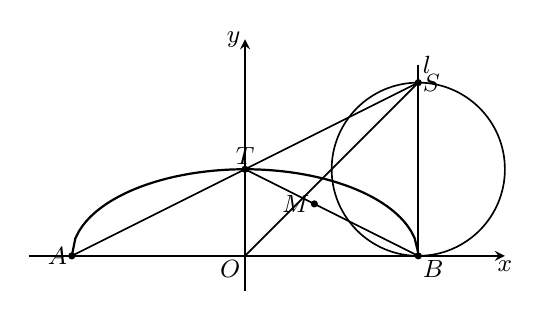
\begin{tikzpicture}[semithick, x=1.1cm, y=1.1cm, every node/.style={inner sep=1.4pt, font=\small}]
  \draw[-stealth] (-2.5,0) -- (3.0,0) node[below] {$x$};
  \draw[-stealth] (0,-0.4) -- (0,2.5) node[left] {$y$};
  \node[below left] at (0,0) {$O$};
  % 上半椭圆
  \draw[thick,domain=-2:2,samples=100] plot (\x,{sqrt(1-\x*\x/4)});
  % 直线 l
  \draw (2,0) -- (2,2.2);
  \node[right] at (2,2.2) {$l$};
  % 点
  \coordinate (A) at (-2,0);
  \coordinate (B) at (2,0);
  \coordinate (S) at (2,2);
  \coordinate (T) at (0,1);
  \coordinate (M) at (0.8,0.6);
  \fill (A) circle (1.3pt);
  \fill (B) circle (1.3pt);
  \fill (S) circle (1.3pt);
  \fill (T) circle (1.3pt);
  \fill (M) circle (1.3pt);
  % 线
  \draw (A) -- (S);
  \draw (T) -- (B);
  \draw (0,0) -- (S);
  \draw (2,1) circle (1);
  % 标注
  \node[left] at (A) {$A$};
  \node[below right] at (B) {$B$};
  \node[right] at (S) {$S$};
  \node[above] at (T) {$T$};
  \node[left] at (M) {$M$};
\end{tikzpicture}
